%--- Header ------------------------------------------------------------

\documentclass[12pt]{article}
\usepackage{draft}
%\usepackage[onehalfspacing]{setspace}

\graphicspath{ {fig/} }
\hyphenation{}

%--- Meta data ---------------------------------------------------------

\usepackage{hyperref}
\hypersetup{
  pdfauthor   ={Jonas Schöley},
  pdftitle    ={},
  pdfsubject  ={},
  pdfkeywords ={},
  hidelinks,
  breaklinks=true,
  colorlinks=false
}

%--- Titlepage ---------------------------------------------------------

\begin{document}

\begin{titlepage}

{\textbf{Title:}
Robustness and bias of excess death estimates in 2020 under varying model specifications
\par\medskip}

{\textbf{Authors:}
Jonas Schöley$^{1}$
\par\medskip}

{\textbf{Affiliations:}\par
$^1$ Interdisciplinary Centre on Population Dynamics, University of Southern Denmark; Odense 5000, Denmark\par
\par\medskip}

{\textbf{Corresponding authors:}\par
Jonas Schöley \href{mailto:jschoeley@health.sdu.dk}{\texttt{jschoeley@health.sdu.dk}}\par
\par\medskip}

{\textbf{Keywords:}
excess deaths; COVID-19; Serfling model; cross-validation; robustness
\par\medskip}

{\textbf{Abstract:}
Various procedures are in use to calculate excess deaths during the ongoing COVID-19 pandemic. Using weekly death counts from 20 European countries, we evaluate the robustness of excess death estimates to the choice of model for expected deaths and perform a cross-validation analysis to assess the error and bias in each model's predicted death counts. We find that the different models produce very similar patterns of weekly excess deaths but disagree substantially on the level of excess. The country ranking of percent excess death in 2020 is sensitive to the exclusion of an exposure variable but otherwise stable across models that do account for population structure. The five-year average death rate model consistently produces the lowest excess death estimates, whereas high excess deaths are produced by the popular five-year average death count and Euromomo models. Cross-validation revealed these estimates to be biased under a causal interpretation of "expected deaths had COVID-19 not happened."
\par\medskip}

% \noindent\begin{tabular}{@{}ll}
% \textbf{Word count:} & 0\\
% \textbf{Figures:} &  0\\
% \textbf{Tables:} & 0\\
% \textbf{References:} & 0
% \end{tabular}

\end{titlepage}

%--- Text --------------------------------------------------------------

\section*{Introduction}

The concept of "excess deaths" became widely known in 2020. Early in the year, international newspapers reported weekly death counts that were notably elevated compared to previous years \citep{EDT2020, NYT2020}. In a situation where tests for COVID-19 were scarce and the underlying cause of death often hard to determine, excess deaths proved to be a rational means of monitoring the direct and indirect mortality impact of the ongoing COVID-19 pandemic with minimal data requirements \citep{Leon2020}.
Since the start of the pandemic, the literature on excess deaths has been growing fast and already features international comparisons and rankings owing to the readily available data on death counts for many countries \citep{Kontis2020, Arolas2021, Rizzi2021, Bilinski2020}.
However, despite the prominence and relevance of the measure, the excess death methodology is far from standardized with different definitions of excess deaths and different models used to estimate an expected death counts against which the excess is judged. This eclectic state of the art begs the questions on robustness and bias of excess death estimates and cross-country comparisons under various analysis strategies.

Given data from 20 European countries, we will assess how excess death measures in the year 2020 vary under different modeling choices for the expected number of deaths. Furthermore, we test the models for bias in their predicted weekly and annual death counts using a time-series cross-validation setup. While the lack of consensus extends beyond the model specification to the very definition of excess deaths, we will focus entirely on the baseline model's impact and define excess as observed minus expected, allowing the measure to be negative.

As the literature on excess deaths in 2020 is dominated by simple average or regression-based approaches, we will restrict our attention to this class of models, focusing on the effect of different specifications. Models based upon multi-year averages are prominently employed by newspapers and statistical offices and featured in the academic literature \citep{Campbell2021, Magnani2020, Michelozzi2020, Modig2020}. While simple and easy to communicate, these procedures do not adjust for time trends in the death counts or rates. This issue is addressed by the Serfling model \citep{Serfling1963}, which in various specifications has been applied to quantify covid related deaths
\citep{Barnard2020, Weinberger2020, Woolf2020, EuroMoMo2020, Arolas2021}.
Generalized additive models relax the strict specifications of the Serfling model and allow for smooth long-term and seasonal effects \citep{Aburto2021, Scortichini2020}. These models may be further elaborated via the inclusion of temperature effects, autoregressive residuals, adjustments for bank holidays, and Bayesian inference \citep{Kontis2020}.

Having chosen 10 model specifications reflecting the heterogeneity in the literature (Table \ref{tab:models}), we probe each model for a tendency to produce high or low estimate of expected and conversely excess deaths, both weekly and total. We ask if the ranking of European countries along the total percentage of excess deaths in 2020 differs under different baseline models, and we identify those countries where there is disagreement about the existence of excess deaths among the models.

When excess death numbers vary by models, the question arises which model to trust. In line with \cite{Kontis2020} and \cite{Modi2020} we argue that the challenge of estimating the expected number of weekly deaths in the year 2020, given that COVID had not occurred, is a classical forecasting challenge, and thus, the models can be validated by testing their predictions on past data. To that end, we construct a cross-validation challenge, where each model is fitted on seven years of weekly death counts and is then tasked to predict the next 52 weeks from that series. The error and bias of any model can then be estimated by comparing the model predictions with the observed data. If a model's predictions tended to over/underestimate weekly deaths in the past, we argue that this model also over/underestimates the expected deaths in 2020 under the counterfactual no-COVID scenario, thereby biasing excess deaths.

\section*{Data and Methods}

\subsection*{Raw and derived data}


To replicate the more elaborate expected death regression models, we collected cross-country data on weekly death counts and population exposure by age and sex, along with information on the timing of public holidays and weekly population-weighted temperature anomalies.

% deaths

Age and sex-specific weekly death counts by country were sourced from the Short-term Mortality Fluctuations (STMF) database \citep{Jdanov2021, Nemeth2021}. We selected all European countries with data going back to at least 2007. As we are using the Mean Absolute Percentage Error (MAPE) measure to report on prediction error, we needed to ensure strictly positive weekly death counts. We thus excluded Estonia, Iceland, and Luxembourg from the analysis and summed deaths into age categories 0 to 65, 65 to 75, 75 to 85, and 85+.

% population exposure

Person-weeks of population exposure by country, sex, and age were derived from mid-year population estimates from the Human Mortality Database \citep{HMD2021}. We summed these estimates into the target age groups and then interpolated over the weeks of a year by fitting a cubic spline and extrapolating linearly to the end of 2020. Integrating the spline over single weeks yielded person-weeks of exposure.

% temperature

Population weighted weekly temperature anomalies were calculated from global gridded temperature \citep{CPC2021} and population data \citep{CIESIN2018}. First, we calculated the average weekly temperature per grid cell from the daily measurements and then weighted these measurements by the population size in the same grid cell. We then selected all grid-cells overlapping with the area of a given country and calculated the country's population-weighted average weekly temperature. By averaging the weekly temperatures over multiple years, we established an expected temperature. A country's weekly population-weighted temperature anomalies were then derived by subtracting this long-term trend from the weekly temperature in a given year.

% holidays

We used the "Nager.Date" software \citep{Hager2021} to determine for each week, year, and country the occurrence and type of a public holiday, distinguishing between Christmas, Easter, New Year, and "other" types of public holidays.

\subsection*{Model choice}

We compare the 10 different models listed in Table \ref{tab:models} in terms of their predicted death counts and their prediction error on historical data. The models are chosen to represent the range of approaches in the literature on excess deaths estimation since the start of the pandemic, from very simple to elaborate, but we do not claim to have exactly replicated any published analysis. All models are either fitted separately for each combination of age and sex or feature interaction terms to the same effect. Further details are given in the supplementary materials. We chose not to include a flu-epidemic variable in any of our models due to endogeneity. Mitigation measures put in place to combat the spread of the Coronavirus also have an impact on the spread of other viruses \citep{Cowling2020, Soo2020}. Therefore, if the expected deaths are to be interpreted as "deaths if COVID had not happened", including post-covid influenza observations is not admissible.

\begin{table}[H]
\small
\caption{Models for weekly expected deaths.}
\label{tab:models}
\begin{tabularx}{\textwidth} {
  >{\raggedright\arraybackslash}X
  >{\raggedright\arraybackslash}X
  >{\raggedright\arraybackslash}X }
\toprule
\textbf{Model} & \textbf{Description} & \textbf{References} \\ \midrule
% Averages
\textbf{Weekly averages}\par
(AVG5c) 5 year average death counts\par
(AVG5r) 5 year average death rates
 &
 simple mean over the weekly deaths counts or death rates in the preceding years
 &
\cite{Modig2020}, \cite{Stang2020}, \cite{Campbell2021}\\ \midrule
% Serfling
\textbf{Serfling Model}\par
(SRFc) without exposures\par
(SRFcem) Euromomo style, i.e. no exposures, no bank holiday coefficient, fitted over 5 years on weeks without flu-activity\par
(SRFr) with exposures
&
Poisson regression on death counts with log-linear long term trend and Fourier-term seasonality
&
\cite{Barnard2020}, \cite{Weinberger2020}, \cite{Woolf2020}, \cite{EuroMoMo2020}, \cite{Arolas2021}
\\ \midrule
% GAM
\textbf{Generalized Additive Model}\par
(GAMr) without temperature anomaly predictor\par
(GAMrt) with temperature anomaly predictor as smoothly varying coefficient over week of year
&
Poisson regression on death counts with log-linear long term trend and cyclical spline seasonality
&
\cite{Aburto2021}, \cite{Scortichini2020}
\\ \midrule
% LGM
\textbf{Latent Gaussian Model}\par
(LGMr) without temperature anomaly predictor\par
(LRMrt) with temperature anomaly predictor as varying coefficient over week of year implemented as cyclic random walk\par
(LGMrt2) same as LRMrt with order 2 autoregressive long term trend and temperature anomaly random walk
&
Bayesian Poisson regression on death counts with autoregressive long term trend and time-varying seasonality
&
\cite{Kontis2020}
\\ \bottomrule
\end{tabularx}
\end{table}

\subsection*{Excess death measures}

We define excess deaths $D^*$ in a given week $w$ and stratum $j$ as
$D_{wj}^* = D_{wj}-\widehat{D}_{wj}$,
where $\widehat{D}$ are the expected deaths under a given model. This definition as a model residual allows capturing eventual mortality displacement effects where a positive excess in part of the year can be followed by negative excess in later weeks. The total number of excess deaths over period $[a,b]$ are given by
$D_{[a,b], j}^* = D_{[a,b], j} - \widehat{D}_{[a,b], j}$,
where
$D_{[a,b], j}=\sum_{w=a}^b D_{wj}$ and
$\widehat{D}_{[a,b], j}=\sum_{w=a}^b \widehat{D}_{wj}$.
Following a common strategy, expected and observed deaths may be summed over strata to estimate the excess at a higher aggregation level \citep{Barnard2020, Aburto2021, Kontis2020, Weinberger2020}.

To facilitate comparisons between countries, we report the weekly percentage increase of observed deaths over expected deaths,
$P_{wj}=\frac{D_{wj}^*}{\widehat{D}_{wj}}$,
the so-called "P-score". For a sequence of weeks $[a,b]$ we calculate the cumulative P-score from the total excess and expected deaths over that period,
$P_{[a,b], j}=\frac {D_{[a,b], j}^*} {\widehat{D}_{[a,b], j}}$.

Any prediction intervals around the quantities above are derived from repeated samples of expected deaths from a Poisson distribution with rate $\widehat{D}_{wj}$. The resulting uncertainty statements should be understood as lower-bound estimates as the Poisson sampling, while easily implemented for any algorithm which predicts death counts, ignores overdispersion in the outcome distribution and uncertainty around model parameters.

\subsection*{Cross-validation}

Time series of weekly death counts and co-variates were split into five cross-validation sets. The training period starts at week 27 of a year and ends after seven fully observed summer to summer seasonal cycles with the beginning of week 8 of a year. After fitting the model, weekly death counts were predicted for 45 weeks following week 8 of the last year in the training set. The starting years for the five cross-validation series were 2007 to 2011. This particular cross-validation setup has been chosen to mirror the task of predicting weekly deaths in 2020, given years of data observed until shortly before the outbreak of the pandemic.

\section*{Results}

% overall variability of excess deaths under different models

Models differed in their estimated level of excess deaths while generally agreeing on the weekly pattern of excess (Figure \ref{fig:excess}). On the country level, the range of weekly and annual percent excess deaths across models was between 5 and 10\%. The average death rate model produced the lowest excess death estimate for all countries, whereas the maximum varied, with the Euromomo style Serfling and the average death count model producing the highest excess in 15 out of 20 countries. Taking Belgium as an example of a region with pronounced mortality, central estimates of excess deaths by the end of 2020 range from 14,968 (.95 PI: 14,472--15,510) under the average death rate model to 21,485 (.95 PI: 21,068--21,851) under a Euromomo style Serfling regression. Consequently, models may disagree regarding the existence of significantly elevated mortality in countries with comparatively few registered COVID deaths. We found such disagreement in Denmark, Finland, and Latvia, where annual P-scores were not significantly elevated under the average death rate model. Norway is the only country under consideration where all models agreed that deaths in 2020 had not been significantly elevated.

\begin{figure}
\caption{Weekly and cumulative excess death percentage as predicted from 10 different models during the year 2020 weeks 8 through 52 for 20 European regions. \emph{Note: Points indicate weekly excess percentages. Cumulative excess percentages are indicated by curves and derived from cumulated observed and expected deaths. The labels refer to the percent excess over the entire analysis period.}}
\label{fig:excess}
\vspace{-1em}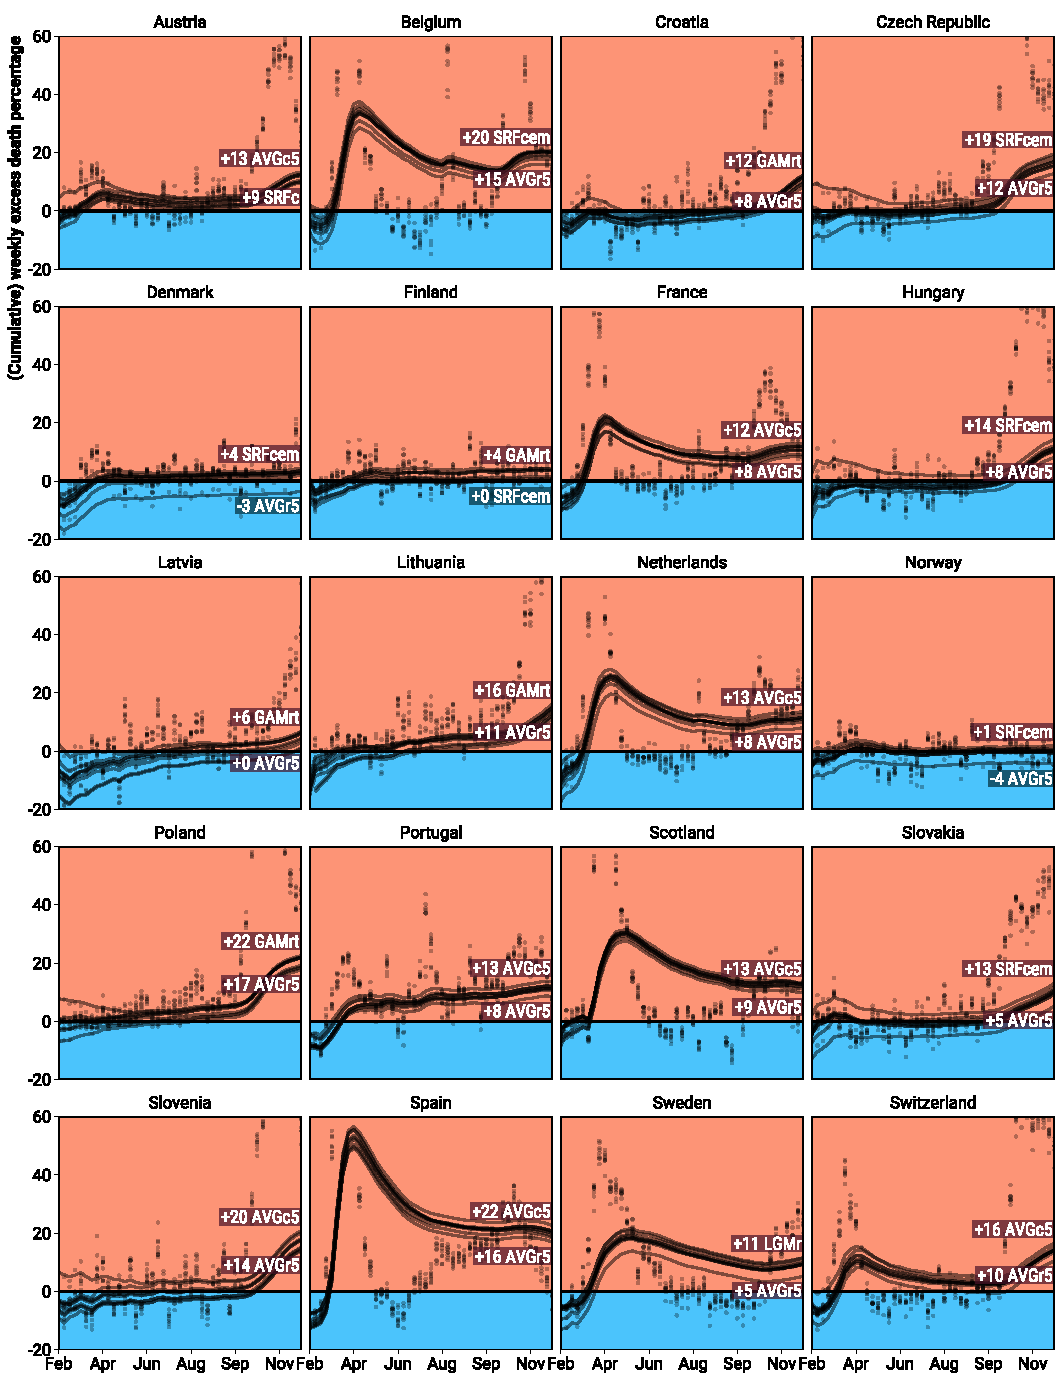
\includegraphics{excess.pdf}
\end{figure}

% country ranking under different models
The ranking of countries along the percent excess deaths in 2020 was largely stable across those models which controlled for population structure (AVGr5, SRFr, GAM*, LGM*) but fluctuated once an exposure variable was excluded (Figure \ref{fig:rank}). All models agreed on the four countries with the highest (Poland, Spain, Belgium, Slovenia) and lowest (Finland, Latvia, Denmark, Norway) annual percent excess. There was substantial disagreement among the exposure-free models (SRFcem, SRFc, AVGc5) regarding the middle ranks with countries moving between quartiles. France and Lithuania are two extreme examples where the European annual P-score rank stretched across three quartiles depending on the model. Within age and sex strata, we observed even more drastic changes in rank across models without exposure variable, whereas the rate-based models largely agreed in their predicted country rankings (Figure \ref{fig:rankstrata}).

\begin{figure}
\caption{Country ranking of excess death percentage during the year 2020 weeks 8 through 52 under 10 different models.}
\label{fig:rank}
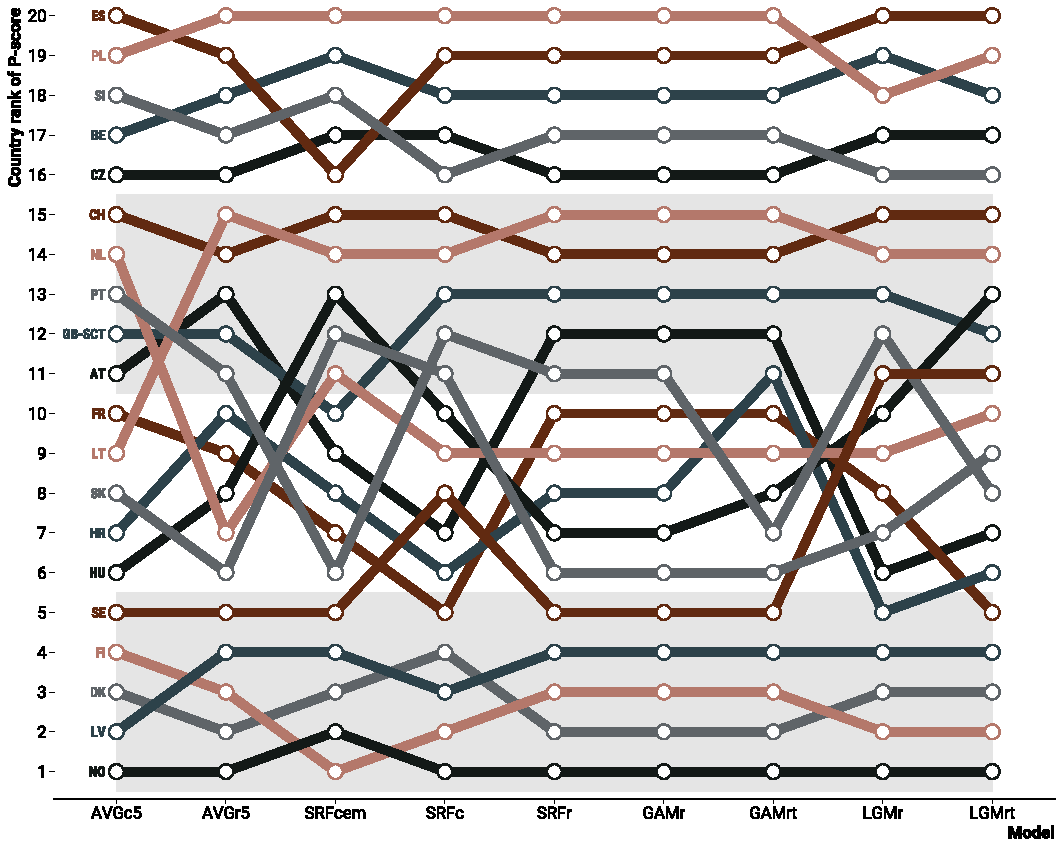
\includegraphics{rank.pdf}
\end{figure}

% prediction deviations from reference model
In Figure \ref{fig:baselinediff}a we compared the 5-year average death count model (AVGc5, the reference) to various other models concerning the expected number of deaths in 2020. The Euromomo Serfling model (SRFcem) and the reference tended to produce the lowest expected death estimates and thus the highest excess death counts, whereas the 5-year average death rate model (AVGr5) gravitated towards the highest expected death counts, with predictions being higher by 3.6 to 5.1\% compared to the reference for half of the countries. The regression models with exposure offset (SRFr, GAM*, LGM*) estimated baseline deaths close to the reference model if somewhat higher, whereas the Serfling model without exposures (SRFc) tended towards substantially higher expected deaths. The Latent Gaussian Models (LGM*) had the highest agreement with the reference, e.g., for half of the countries, the sophisticated model LGMrt2 produced estimates within -0.7 to 1.1\% of the basic average death count prediction. Similar results were found for predictions of total deaths by sex and age strata within a country, albeit with higher variability of the percentage differences for any given model (Figure \ref{fig:baselinediff}b).

\begin{figure}
\caption{Percent differences of predicted death counts from various models against the 5-year average weekly death prediction. \emph{Note: The prediction differences were summarised across countries and, where applicable, weeks and strata by the 0.25, 0.5, and 0.75 quantiles.}}
\label{fig:baselinediff}
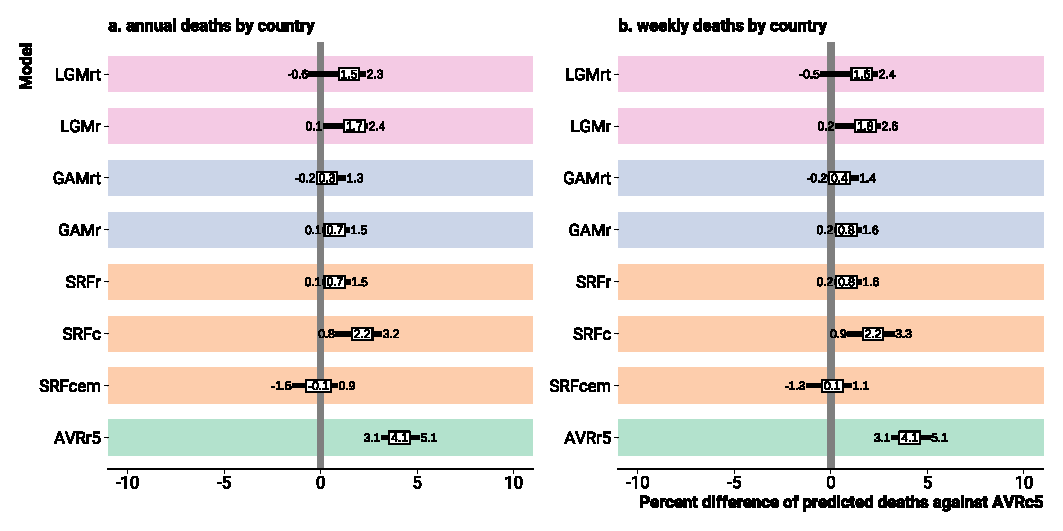
\includegraphics{baselinediff.pdf}
\end{figure}

Percentage differences of predicted weekly death counts against the reference model are shown in Figures \ref{fig:baselinediff}c and d. Again, the 5-year average death rate model tended to produce the highest estimates, with half of the weekly predicted counts being at least 3.8\% above those from the reference. The regression models, on average, predicted fewer deaths than reference, with the Euromomo Serfling model featuring especially low weekly expected deaths. Note, however, that these percentage differences varied considerably over countries and strata due to the high variability of the weekly predictions.

% cross validation results

\begin{figure}
\caption{Distribution of test set errors and bias for predicted death counts. \emph{Note: The MAPE (bold) and the MPE were summarised across countries and, where applicable, weeks and sex*age strata by the 0.25, 0.5, and 0.75 quantiles.}}
\label{fig:biaserror}
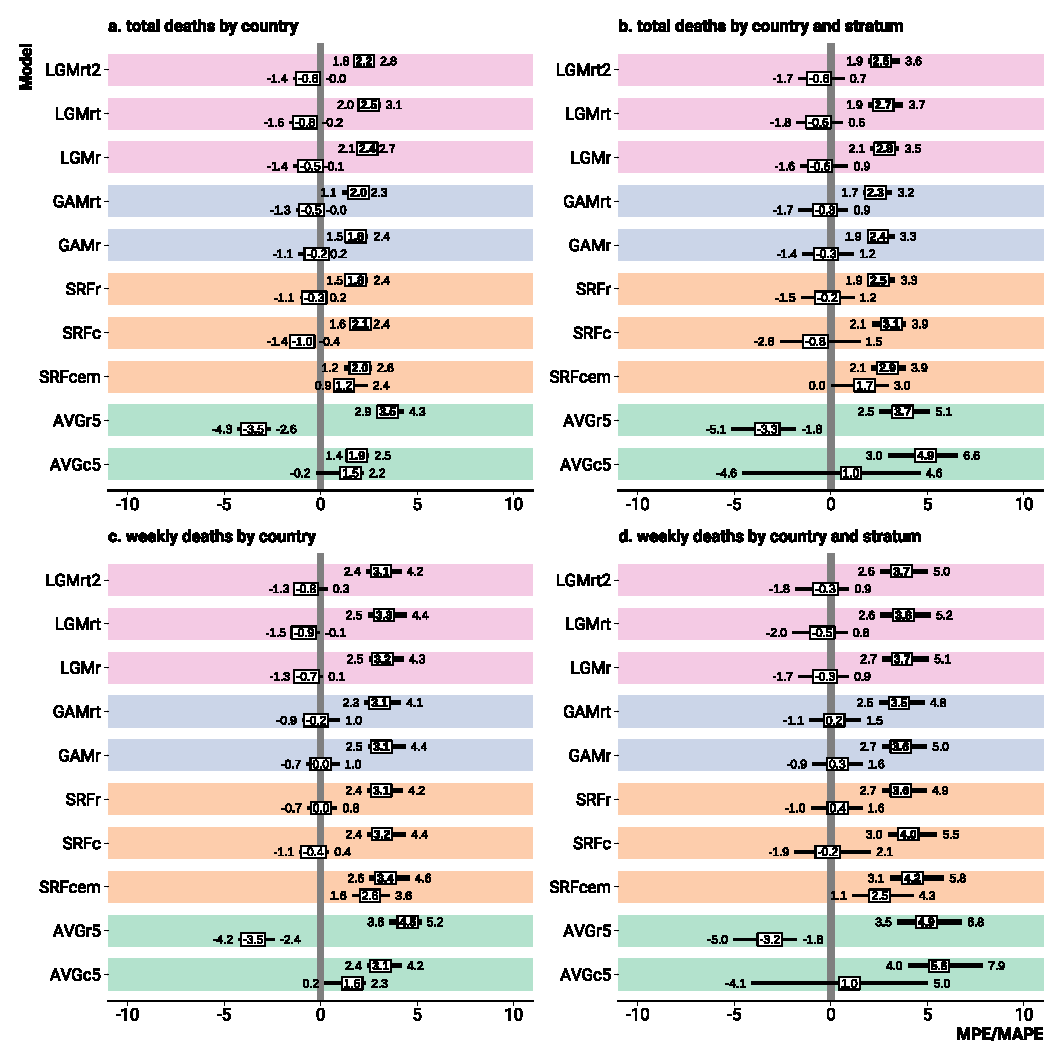
\includegraphics{errorbias.pdf}
\end{figure}

The cross-validation study confirmed the substantial biases of the Euromomo Serfling regression and the 5-year average death rate and count models (Figure \ref{fig:biaserror}a--d). While the average rate model (AVGr5) consistently displayed the highest propensity among all models to overestimate deaths on four different prediction tasks, the average count (AVGc5) and the Serfling Euromomo models (SRFcem) underestimated deaths. Regression models with exposure offset were comparatively unbiased.

When predicting country-level total deaths over weeks 8 through 52 of a year, the median MAPE on the test set ranged from 1.8\% for the best performing regression models (SRFr, GAMr) to 3.5\% for the average death rate model. Notably, the MAPE from the 5-year average death count model was comparable to the error of the best-performing regression models when predicting annual or weekly deaths on the country level (Figures \ref{fig:biaserror}a and c). However, when predicting deaths by sex and age strata, the regression models performed substantially better than either the average rate or count model, with little difference between the various regression specifications (Figures \ref{fig:biaserror}b and d). Cross-validation errors for all models increased by approximately 1 to 2 percentage points going from annual to weekly predictions.

\section*{Discussion}

No matter the chosen model, in 2020, excess deaths across Europe have reached levels not seen since World War 2. Other inferences, however, are less robust to the choice of model. Depending on how the expected deaths were calculated, one may have either Poland, Spain, or Belgium as the worst affected country, Denmark may or may not have had significantly elevated death counts, annual deaths among Slovenian males ages 85+ may be increased by as little as 4\% to as much as 15\%, and death counts following the first wave of the pandemic may have returned to expected levels or dropped into a “mortality deficit.” Thus, short of a standard procedure of specifying expected deaths, robustness checks are crucial. In the simplest case, such a check could be based upon expected deaths via five-year average death rates and alternatively the Serfling Euromomo model, as we found these two approaches to have opposite biases, with predictions from other methods falling in-between.

The Euromomo model is designed to predict death counts as expected under exceptionally mild seasonal mortality increases, thus resulting in high estimates of excess death. While this makes the Euromomo approach very useful for monitoring influenza-related mortality, the baseline is biased if interpreted as "expected deaths in the absence of the COVID-19 pandemic", as the typical seasonal increase in deaths is not as shallow as predicted under Euromomo. The technical reason for the low Euromomo predictions during fall and winter is the exclusion of weeks with likely influenza activity from the model fitting. If the modeling goal is mortality forecasting, as under the counterfactual no-COVID scenario, then fitting seasonal regression models over all weeks of a year reduces the bias in the forecasted death counts.

A lack of adjustment for continuous mortality improvements, as have been observed across Europe up until 2020 \citep{Leon2011, Aburto2021a}, explains the tendency of the average death rate model towards low estimates of excess. By simply averaging declining death rates over time, one overestimates expected mortality for the current year, thus underestimating excess. Claims of no excess deaths based upon averaged weekly death rates should therefore be checked for robustness against the inclusion of a time trend.

Two opposing time-trends explain the bias of the ubiquitous average weekly death count model: increasing deaths due to population aging and decreasing deaths due to mortality improvements. As the model adjusts for neither trend, it may be biased in either direction, depending on the relative size of either effect in any given country, although we found a slight tendency towards high excess death estimates across Europe. The lower overall bias when averaging counts instead of rates suggests that errors due to non-adjusted time trends cancel to some degree, showing that an incomplete adjustment to trends can be worse than no adjustment at all.

All seasonal regression models exhibited similar biases given that changing population structure and rates of mortality improvement were adjusted for. The inclusion of temperature effects or autoregressive structures did not consistently improve cross-validation error. A major challenge faced by every model is to estimate the magnitude of the seasonal effect. In the absence of information about influenza activity, all models just predicted an average seasonality for the following Fall and Winter, possibly with minor temperature adjustments. Whether or not an influenza predictor should be included when estimating excess deaths over the COVID-19 pandemic depends on the purpose of the analysis: causal inference or mortality monitoring. A causal estimate of the direct and indirect effects of the pandemic on overall mortality can not accommodate observed influenza activity past the beginning of the pandemic as this variable is itself influenced by the "treatment," i.e., COVID-19 and associated mitigation measures. In a counterfactual world where the COVID-19 pandemic did not happen, influenza activity throughout 2020 may have been different. For mortality monitoring purposes, however, the inclusion of an influenza predictor is admissible as the question is whether the currently observed death counts are unusual given the currently observed levels of influenza.

How many deaths would we have expected in 2020 if this would have been a typical year? Our definition of expected deaths allows to discriminate between suitable and unsuitable models on empirical grounds: We want a model that excels at short-term forecast of weekly death counts. While robustness checks are a pragmatic way to deal with the reality of many seemingly equivalent analysis strategies, models of expected deaths are not beyond scrutiny. They can and should be put to the test.

\clearpage

%--- Bibliography ------------------------------------------------------

\bibliography{refs.bib}

\clearpage

%--- Appendix ----------------------------------------------------------

\renewcommand\thefigure{S.\arabic{figure}}
\setcounter{figure}{0}

\begin{appendix}

\section*{Supplementary materials}

\subsection*{Model description}

\begin{tabular}{llllll}
$i$ & observation within a country & $\alpha$ & intercept & $j$ & sex$\times$age stratum \\
$t$ & weeks since start of data series & $\beta, \zeta$ & time trend coefficients & $j[i]$ & stratum of observation $i$ \\
$w$ & weeks since start of epi-year & $\gamma$ & seasonality coefficient & $D$ & death count \\
$H$ & public holiday indicator & $\delta$ & holiday coefficient & $E$ & person-weeks exposure \\
$T$ & temperature anomaly & $\nu$ & temperature anomaly coef. & $f,g$ & smooth functions of time
\end{tabular}

\vspace{1em}

We fit the \emph{Serfling with exposures} (SRFr) via

\begin{equation}
\begin{aligned}
  D_i \sim& \text{Pois}(\lambda_i) \\
  \log \lambda_i =& \alpha_{j[i]} + \beta_{j[i]}t_i + \\
& \gamma_{1,j[i]}\sin\left(\frac{2\pi}{52}w_i\right) +
  \gamma_{2,j[i]}\cos\left(\frac{2\pi}{52}w_i\right) +
  \gamma_{3,j[i]}\sin\left(\frac{2\pi}{26}w_i\right) +
  \gamma_{4,j[i]}\sin\left(\frac{2\pi}{26}w_i\right) + \\
 & \delta_{j[i]}H_i + \log E_i.
\end{aligned}
\label{eq:srfr}
\end{equation}

Omitting the term $\log E_i$ from (\ref{eq:srfr}) yields the \emph{Serfling without exposures} (SRFc) model. For the \emph{Euromomo style Serfling model} (SRFcem) we dropped the exposure, holiday and half year seasonal cycle from (\ref{eq:srfr}) and only fitted the model over a five year period on weeks 15 through 26 and 36 through 45.

The \emph{Generalized Additive Model with temperature anomaly} (GAMrt) allows for non-parametric, smooth seasonal effects and adjusts for the effect of extreme temperature on weekly death counts. We specify the model as

\begin{equation}
  \begin{aligned}
    D_i \sim& \text{Pois}(\lambda_i) \\
    \log \lambda_i =& \alpha_{j[i]} + \beta_{j[i]}t_i + f_{j[i]}(w_i) + \nu_{w[i]} T_i + \delta_{j[i]}H_i + \log E_i,
  \end{aligned}
  \label{eq:gamrt}
\end{equation}

where $f_{j[i]}(w_i)$ is a stratum specific seasonality term implemented as a cyclical penalized spline, and $\nu_{w[i]}=g(w_i)$ is the temperature anomaly coefficient varying smoothly over week of year in a cyclical fashion. For the \emph{Generalized Additive Model without temperature anomaly} (GAMr) we omitted this term.

The \emph{Latent Gaussian model with temperature anomaly} (LGMrt) follows the specification by \cite{Kontis2020}. The model is fitted separately by age group and sex and in the following we omit the subscript $j[i]$.

\begin{equation}
  \begin{aligned}
    D_i \sim& \text{Pois}(\lambda_i) \\
    \log \lambda_i =& \alpha + \beta t_i +
    \zeta_{t[i]} + \gamma_{t[i]} +
    \nu_{w[i]} T_i + \delta H_i + \log E_i.
  \end{aligned}
  \label{eq:lgmrt}
\end{equation}

The model features three components modeling the weekly time series of death rates: $\beta t_i$ is a simple log-linear trend over time, $\zeta_{t[i]} \sim \text{Normal}(\phi \zeta_{t[i]-1}, \sigma^2_\zeta)$ is a first order autoregressive trend, and $\gamma_{t[i]}$ is a seasonal random effect under the prior that the summed effect of every consecutive series of 52 weeks on mortality is distributed as $\sum_{s=0}^{51} \gamma_{t[i]+s} \sim \text{Normal}(0, \sigma^2_\gamma)$, thus allowing for a varying magnitude of seasonality over years.

[To be continued]

\subsection*{Supplementary figures}

\begin{figure}
\caption{Rolling origin five-fold cross-validation setup mirroring the task of predicting weekly deaths past the beginning of the COVID pandemic given pre-pandemic data.}
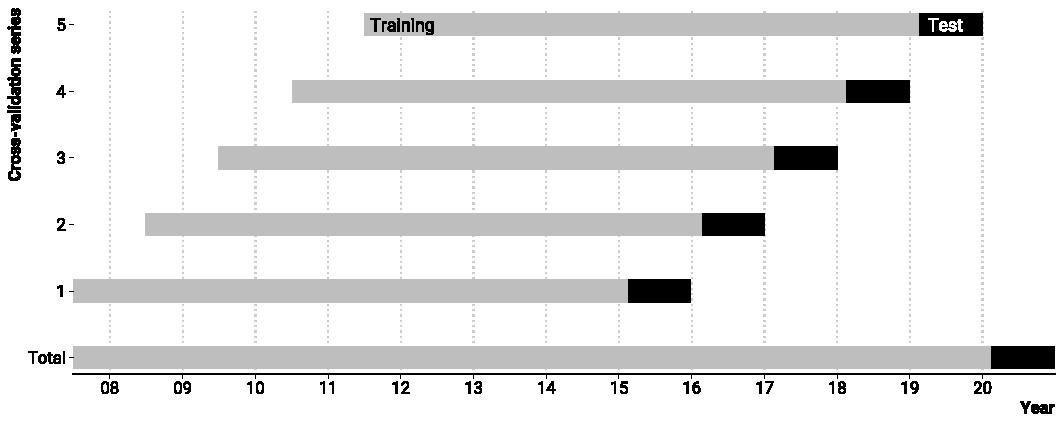
\includegraphics{cvsetup.pdf}
\end{figure}

\begin{figure}
  \caption{Population weighted weekly temperature anomaly by country.}
  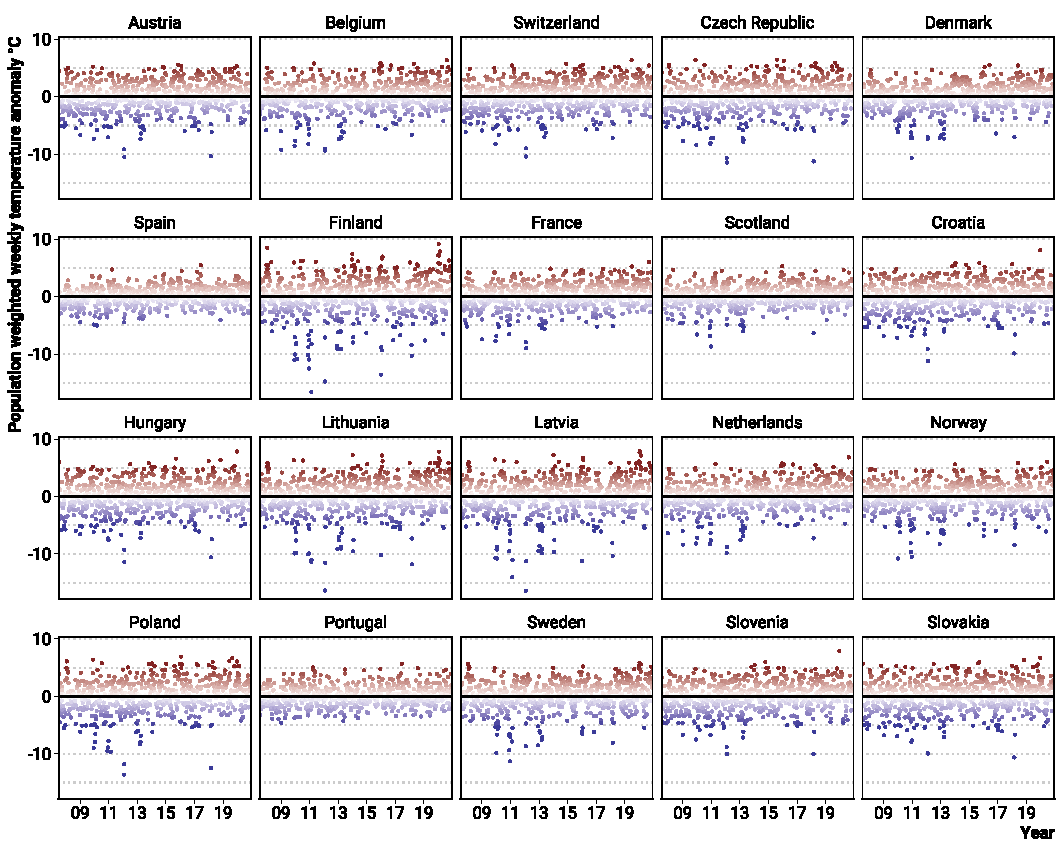
\includegraphics{tanomaly.pdf}
  \end{figure}

% Female excess plots

\begin{figure}
\caption{
Female percent excess deaths for ages 0 to 65 as predicted from 10 different models during the year 2020 weeks 8 through 52 for 20 European regions.}
\label{fig:excessf0to65}
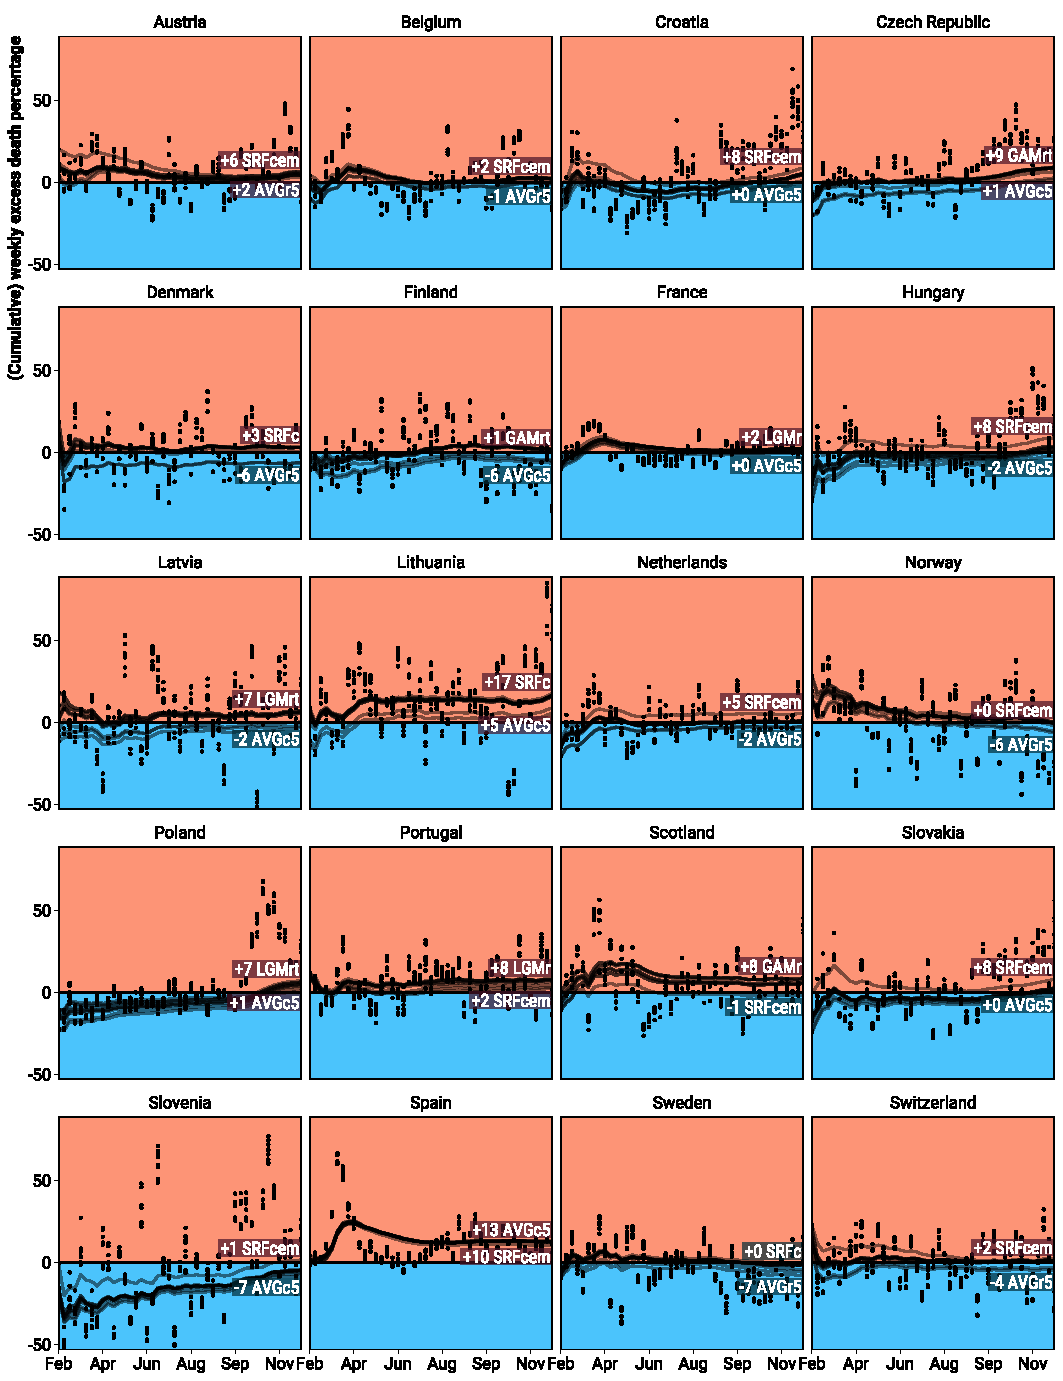
\includegraphics{excess_female__0_65_.pdf}
\end{figure}

\begin{figure}
\caption{
Female percent excess deaths for ages 65 to 75 as predicted from 10 different models during the year 2020 weeks 8 through 52 for 20 European regions.}
\label{fig:excessf65to75}
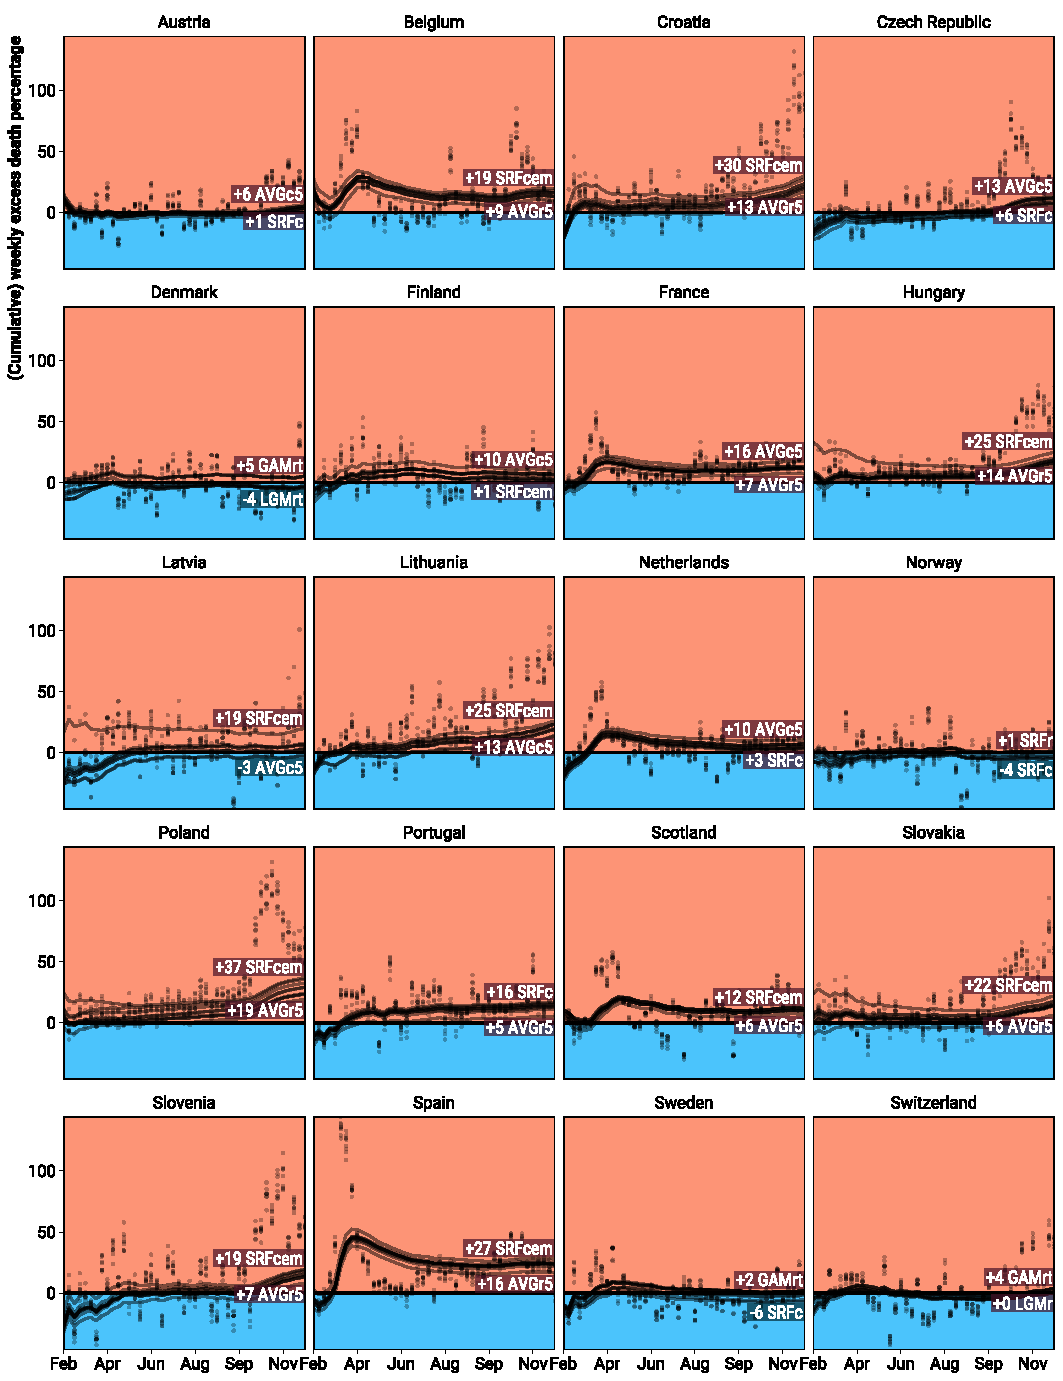
\includegraphics{excess_female__65_75_.pdf}
\end{figure}

\begin{figure}
\caption{
Female percent excess deaths for ages 75 to 85 as predicted from 10 different models during the year 2020 weeks 8 through 52 for 20 European regions.}
\label{fig:excessf75to85}
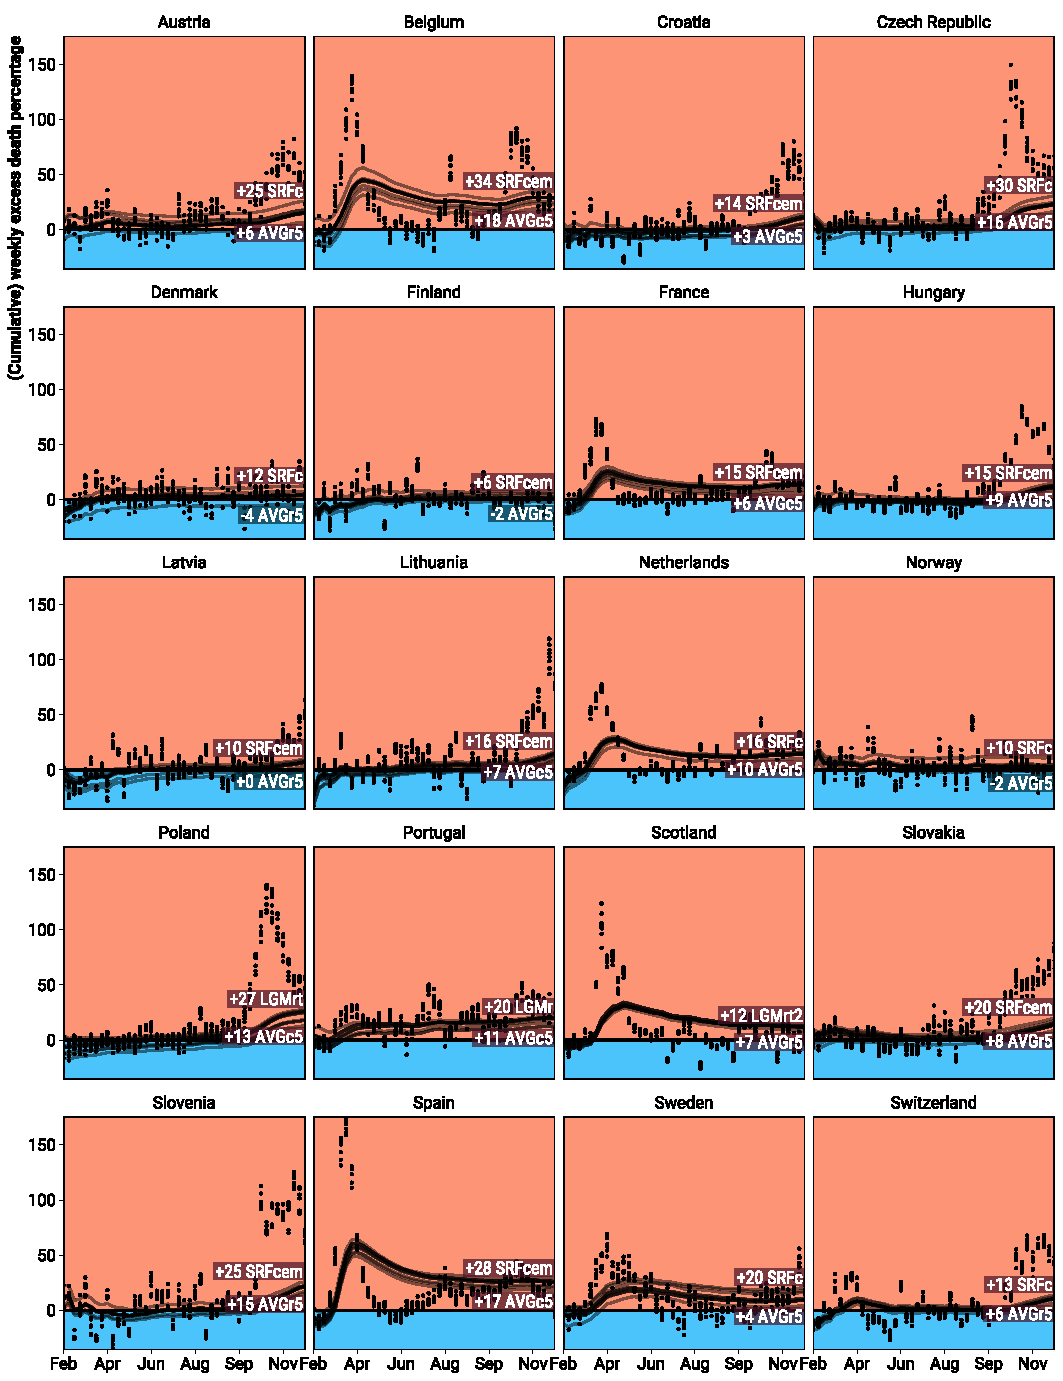
\includegraphics{excess_female__75_85_.pdf}
\end{figure}

\begin{figure}
\caption{
Female percent excess deaths for ages 85+ as predicted from 10 different models during the year 2020 weeks 8 through 52 for 20 European regions.}
\label{fig:excessf85plus}
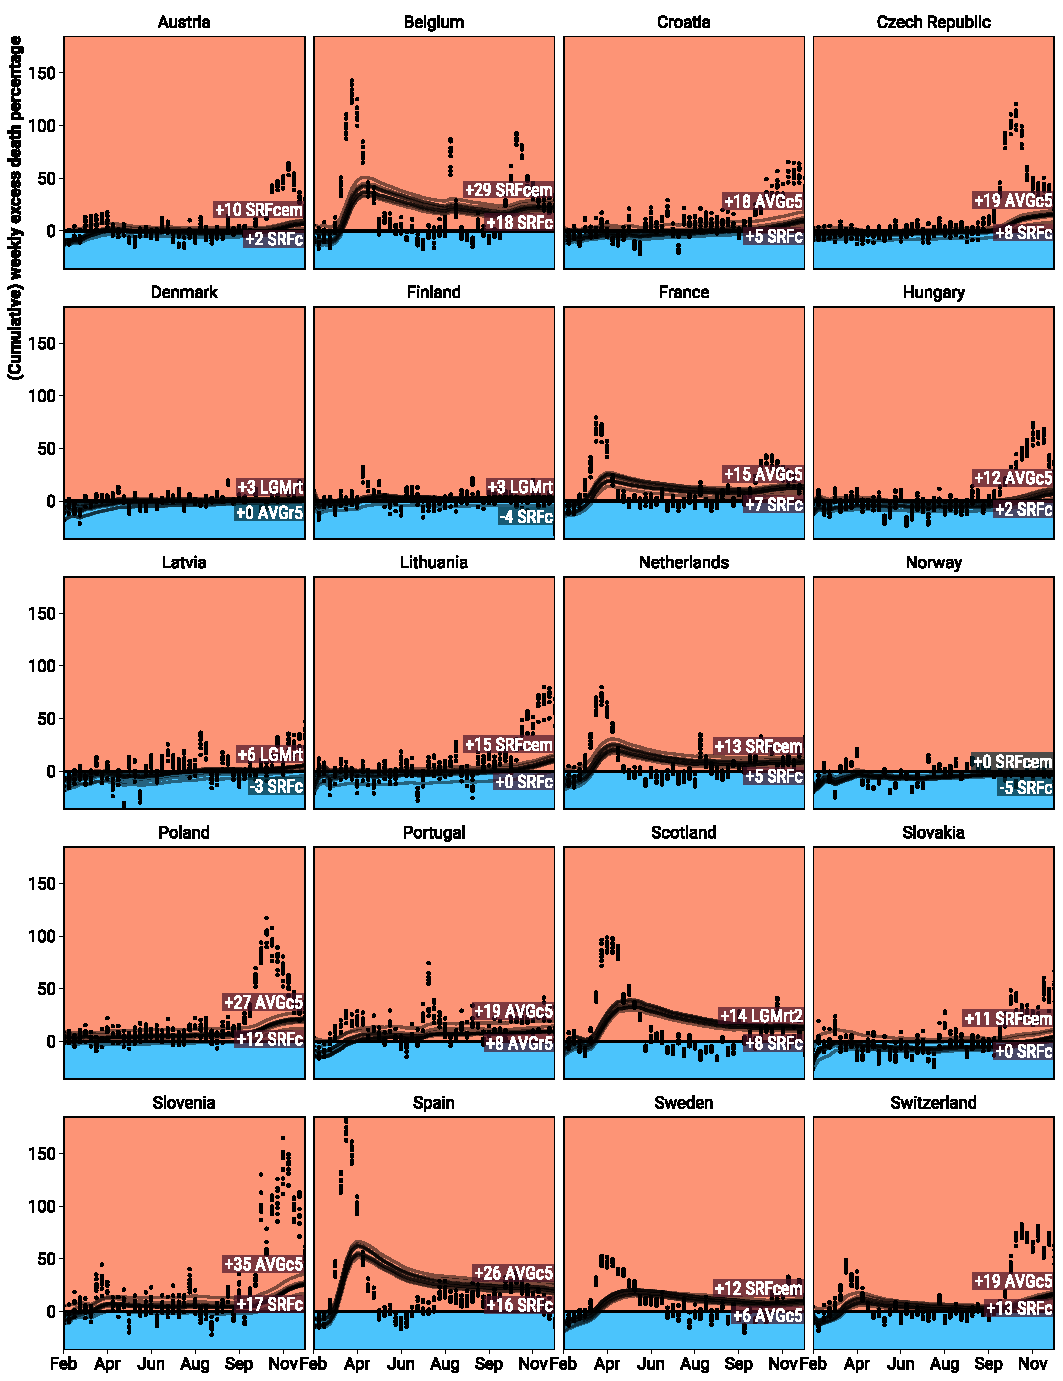
\includegraphics{excess_female__85_inf_.pdf}
\end{figure}

% Male excess plots

\begin{figure}
\caption{
Male percent excess deaths for ages 0 to 65 as predicted from 10 different models during the year 2020 weeks 8 through 52 for 20 European regions.}
\label{fig:excessm0to65}
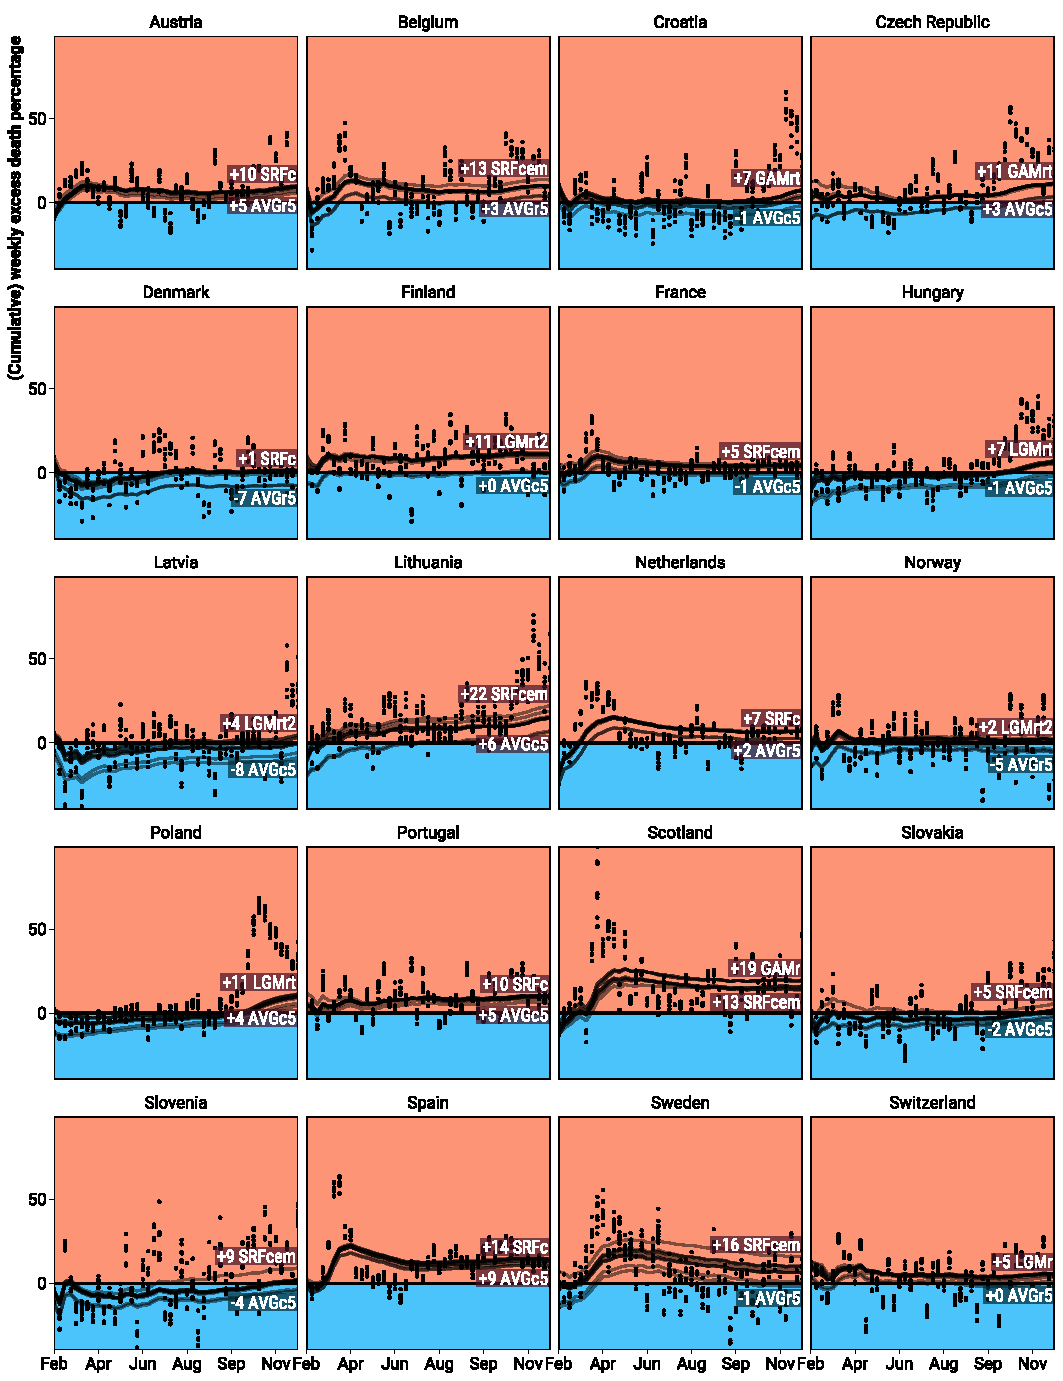
\includegraphics{excess_male__0_65_.pdf}
\end{figure}

\begin{figure}
\caption{
Male percent excess deaths for ages 65 to 75 as predicted from 10 different models during the year 2020 weeks 8 through 52 for 20 European regions.}
\label{fig:excessm65to75}
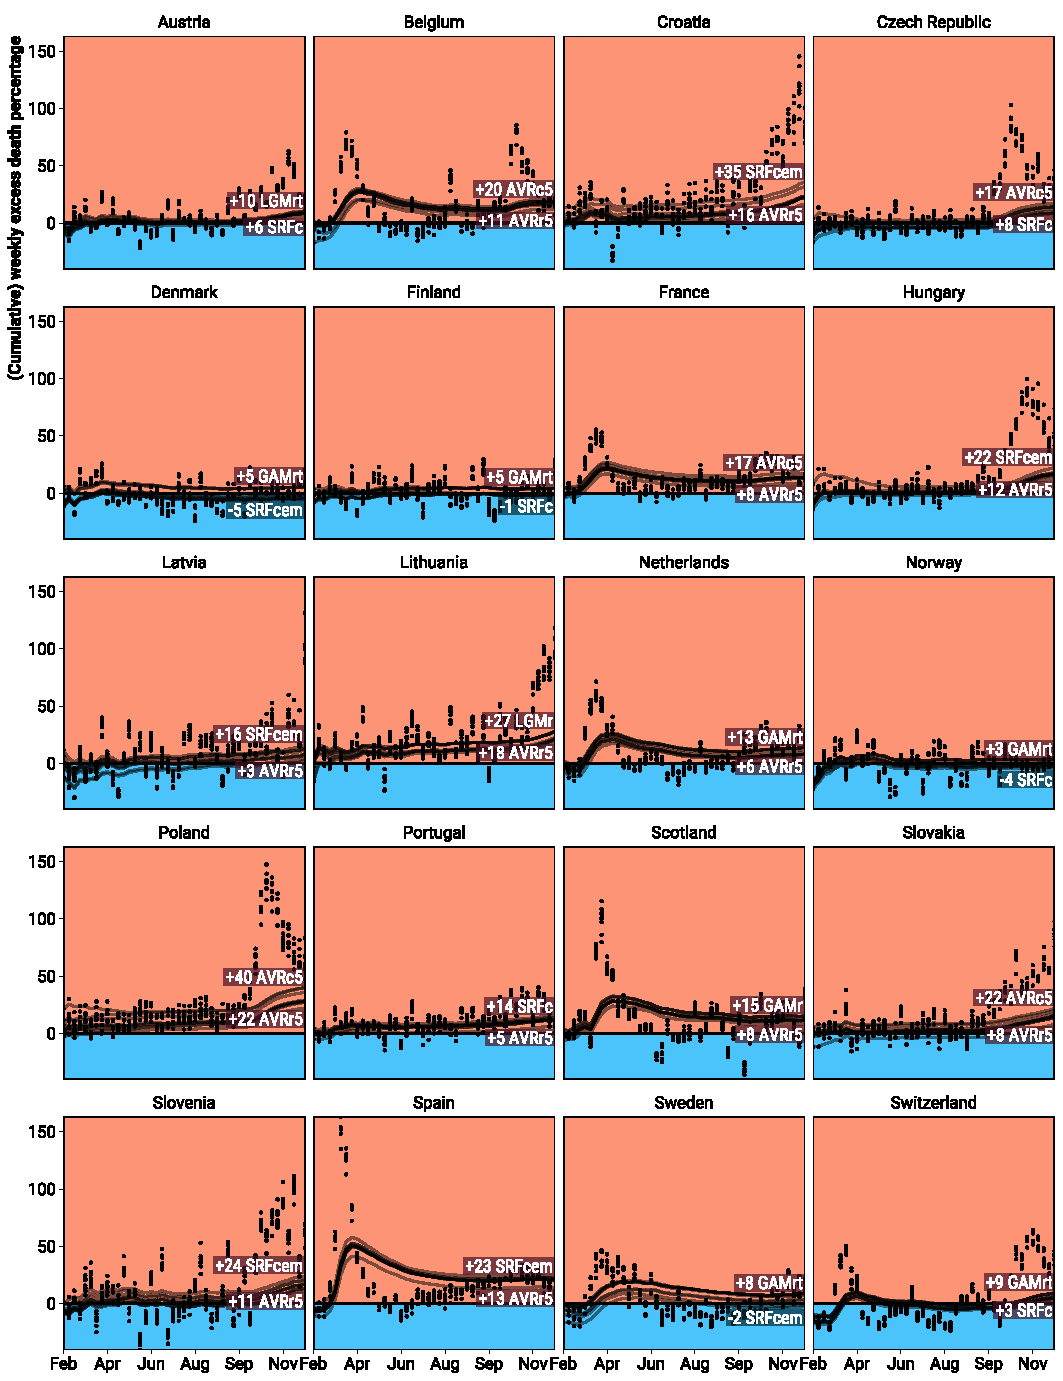
\includegraphics{excess_male__65_75_.pdf}
\end{figure}

\begin{figure}
\caption{
Male percent excess deaths for ages 75 to 85 as predicted from 10 different models during the year 2020 weeks 8 through 52 for 20 European regions.}
\label{fig:excessm75to85}
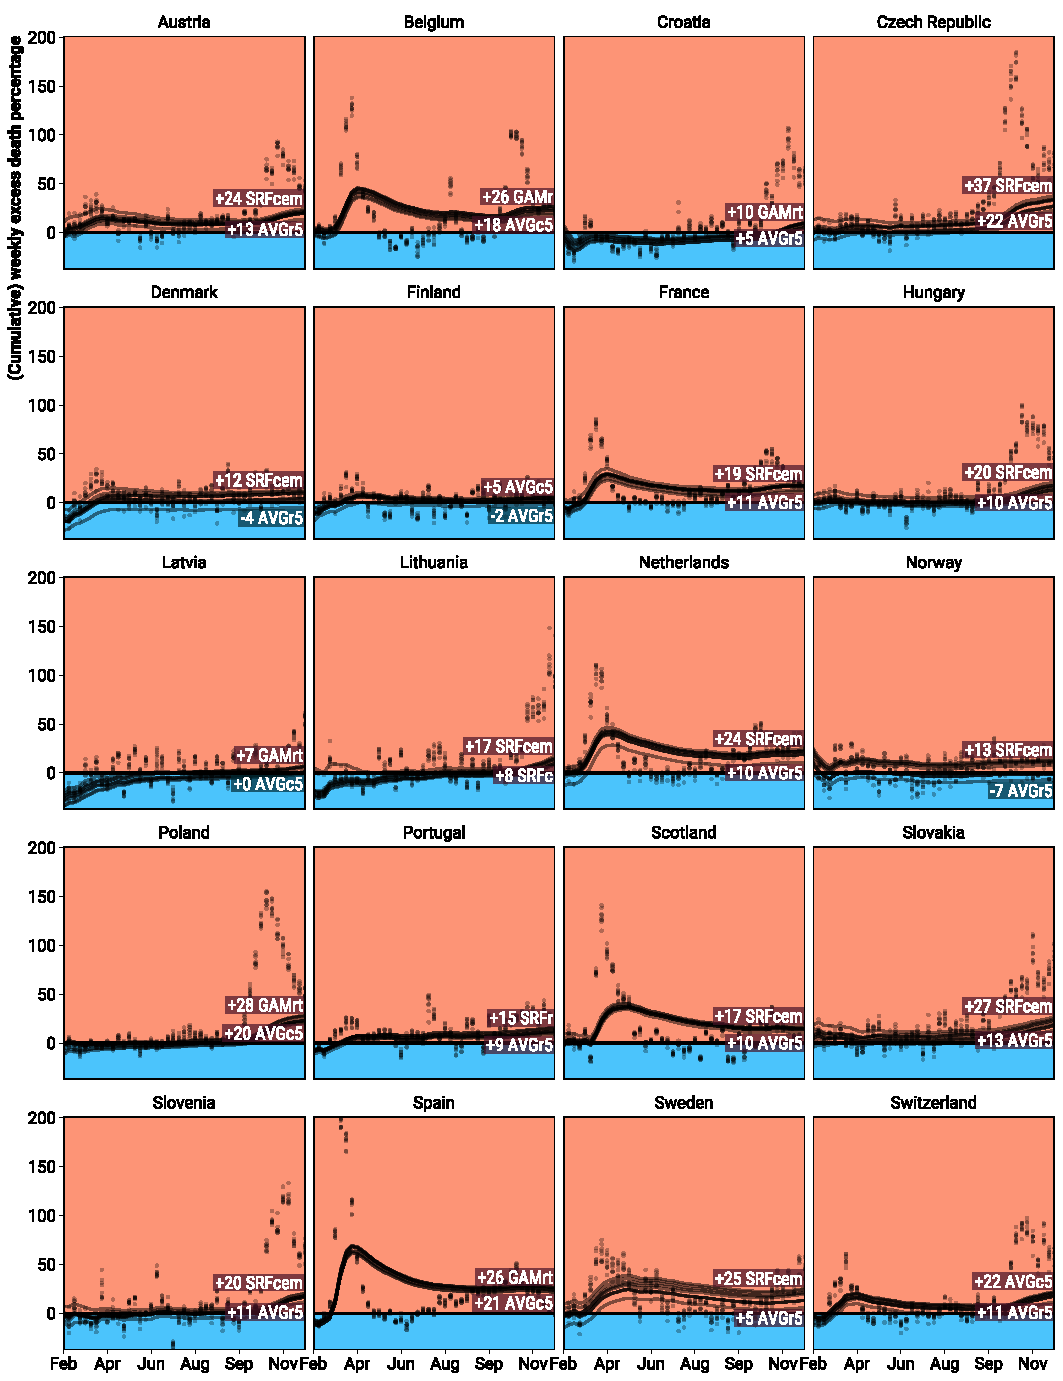
\includegraphics{excess_male__75_85_.pdf}
\end{figure}

\begin{figure}
\caption{
Male percent excess deaths for ages 85+ as predicted from 10 different models during the year 2020 weeks 8 through 52 for 20 European regions.}
\label{fig:excessm85plus}
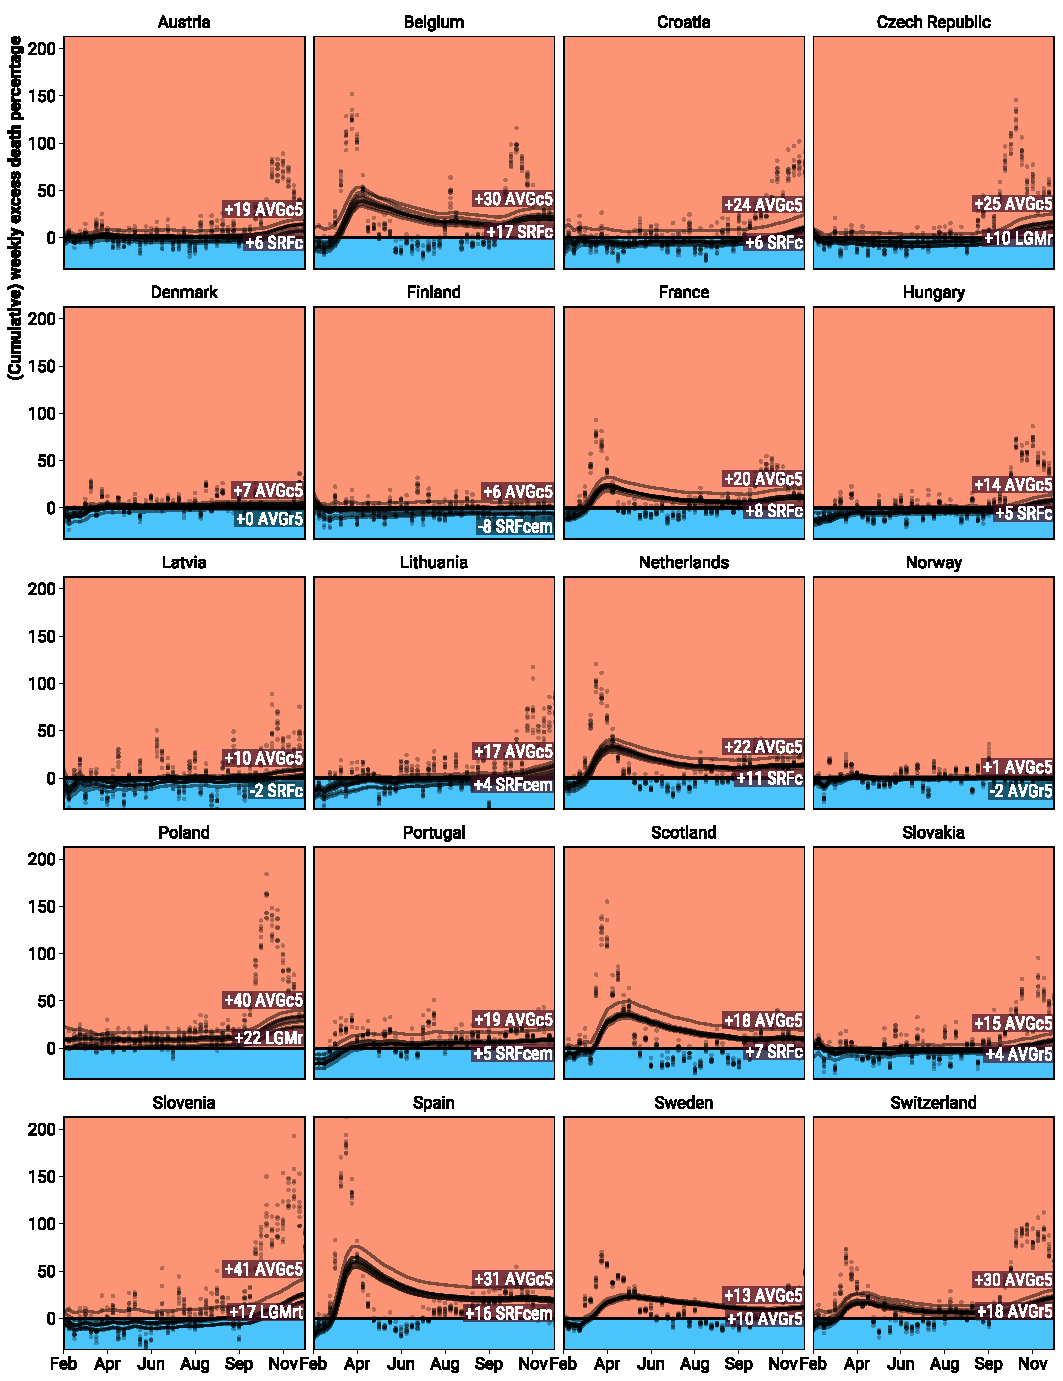
\includegraphics{excess_male__85_inf_.pdf}
\end{figure}

% P-score country rank by stratum

\begin{figure}
\caption{Within-stratum country ranking of excess death percentage during the year 2020 weeks 8 through 52 under 10 different models.}
\label{fig:rankstrata}
\vspace{-1em}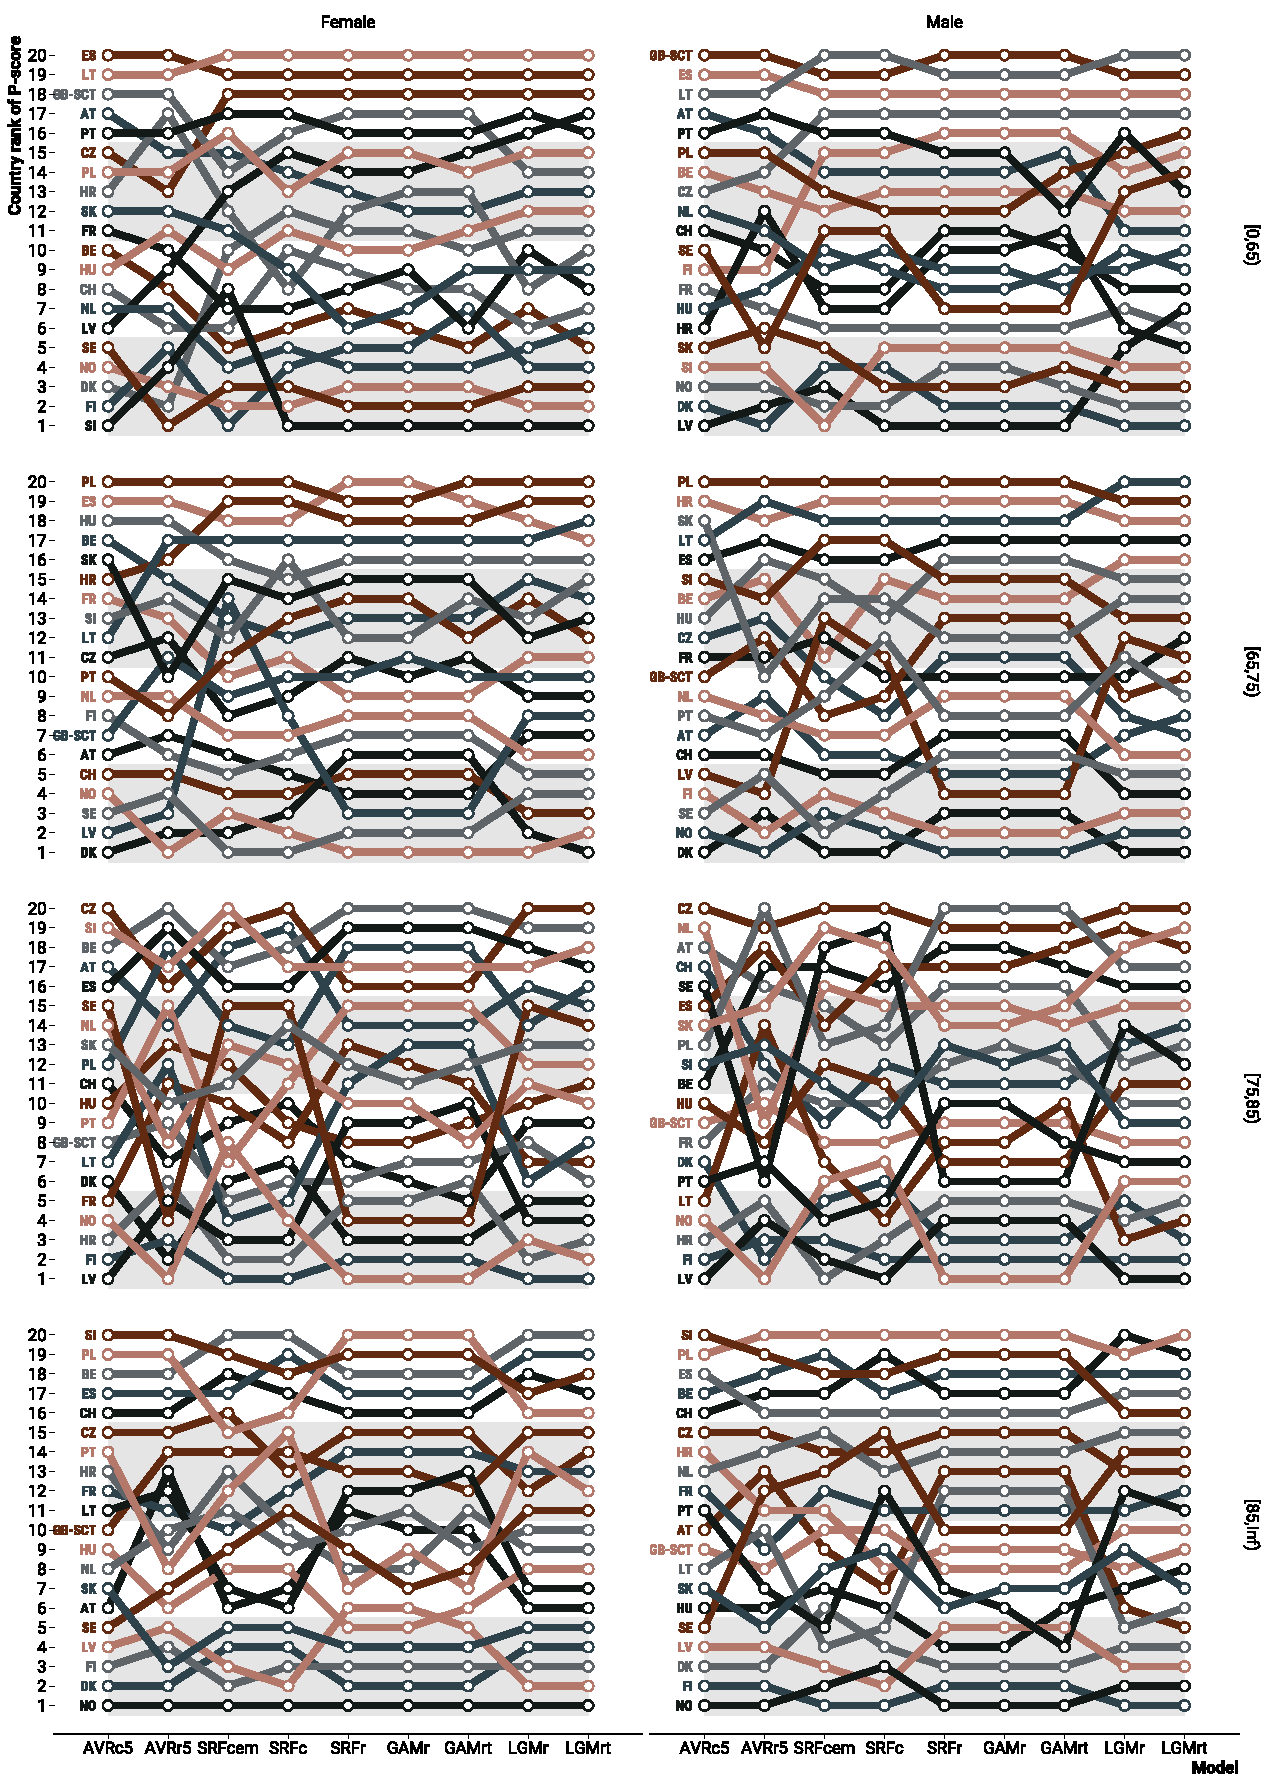
\includegraphics{rank_strata.pdf}
\end{figure}

\end{appendix}

\end{document}
